%% Latex Template for 16-720J student reports
%% You should maintain the template format wherever practical
%% Gary Overett 2015

\documentclass[12pt]{article}
\usepackage{amsmath}
\usepackage{amssymb}
\usepackage{amsthm}
\usepackage{amscd}
\usepackage{amsfonts}
\usepackage{graphicx}
\usepackage{subcaption}
\usepackage{fancyhdr}
\usepackage{tablefootnote}
\usepackage{subcaption}
\usepackage[table]{xcolor}
\usepackage{array,multirow}
\usepackage{hyperref}
\usepackage{enumerate}
\usepackage{bm}

\usepackage[framed,numbered]{mcode}

% \usepackage{listings}
% \lstset{language=Matlab}
% \lstset{breaklines}
% \lstset{extendedchars=false}

\topmargin-2cm
\textheight+23cm

\textwidth6.5in

\setlength{\topmargin}{0in} \addtolength{\topmargin}{-\headheight}
\addtolength{\topmargin}{-\headsep}

\setlength{\oddsidemargin}{0in}

\oddsidemargin  0.0in \evensidemargin 0.0in 

\newcounter{list}

\begin{document}

\title{16720J: Homework 2 - Bag-of-Words for Scene Classification}

\author{Name - WENBO ZHAO (WZHAO1)}

\maketitle

\setcounter{section}{2}

\section{Warming up with some theory (10pts)}

\renewcommand{\thesubsection}{\bf Question \arabic{section}.\arabic{subsection}}

\subsection{(3pts, 2-3 lines)}

Given an $N \times N$ image, and an $h \times h$ Gaussian filter, we can convolve the image and the filter in $O(h)$
time by first convolving the image horizontally with an $h \times 1$ filter and then convolving vertically with a $1 \times h$ filter.  

% see the slides on convolution for the answer

\subsection{(2pts, 2-3 lines)}
\label{sub:bag-of-words}
No. Because \emph{bag-of-words} takes the features of images (by filtering or feature points extraction) and clusters them into a visual words dictionary. The representation of images is converted to mapping each pixel to the dictionary. After histing the frequency of each visual word in the mapped images, we get totally statistic features, neglecting their spatial distribution information.

\subsection{(5 pts, 2-3 lines)}

Because we want to use a bank of different filters to extract the local texture information of an image in a sampling-reasonable way, but at the same time depressing the noise as much as possible. 

\section{Representing the World with Visual Words (40pts)}
\label{repviswords}

\subsection{(5 pts, 3-4 lines) Theory:}

There are 3 groups of filters, 11 in each group. For one group:

The first 3 filters are ``\emph{Gaussian}'' filters, they smooth the noise in the image.

The second 4 filters are ``\emph{LoG}'' filters, they smooth the noise and detect the edges in the image.

The third 4 filters are ``\emph{Derivative of Gaussians}'' filters, they pick up the ``\emph{gradient change in a direction}'' in the image.

\subsection{(15 pts)}

Coding question, put your implementation in \verb+baseline/getFilterBankAndDictionary.m+

\lstinputlisting{./code/getFilterBankAndDictionary.m}

\subsection{(5 pts, 3-4 lines) Theory}
If the visual words dictionary is too small, it cannot fully represent the filtered responses of images in the training set, thus cannot distinguish the filtered responses well. Contrarily, if the dictionary goes too large, similar responses can be represented by different words, it lacks generalization and is sensitive to noise. It also yields high mapping dimension and exhaustive computation.

\subsection{(15 pts)}

Coding question, put your implementation in \verb+baseline/getVisualWords.m+

\lstinputlisting{./code/getVisualWords.m}

\section{Building a Recognition System (95pts)}

\subsection{(10 pts)}

Coding question, put your implementation in \verb+baseline/getImageFeatures.m+

\lstinputlisting{./code/getImageFeatures.m}

\subsection{Extra credit (5 pts 2-3 lines) Theory:}
Because by normalizing all histograms by the total number of features in the image, we first make the histograms from different sublayers and subcells comparable, and we also reduce computational cost.

\subsection{Extra credit (5 pts 2-3 lines) Theory}

Because by weighting different layers inversely proportional to the cell size at the layer, we penalize matches found in larger cells that might induce increasingly dissimilar features.

\subsection{(20 pts)}

Coding question, put your implementation in \verb+baseline/getImageFeaturesSPM.m+

\lstinputlisting{./code/getImageFeaturesSPM.m}

\subsection{(10 pts)}

Coding question, put your implementation in \verb+baseline/distanceToSet.m+

\lstinputlisting{./code/distanceToSet.m}

\subsection{(5 pts)}

Coding question, put your implementation in \verb+baseline/createHistograms.m+

\lstinputlisting{./code/createHistograms.m}

\subsection{(5 pts)}

Coding question, provide any helper code you wrote for this section and list the files here. Also make sure your
\verb+.mat+ is included in your submission.

\lstinputlisting{./code/trainSystem.m}

\subsection{(10 pts)}

Coding question, put your implementation in \verb+baseline/knnClassify.m+

\lstinputlisting{./code/knnClassify.m}

\subsection{(10 pts)}
\label{confusionMatrix}

Coding question, put your implementation in \verb+evaluateRecognitionSystem.m+

\lstinputlisting{./code/evaluateRecognitionSystem.m}

Verbatim copy of your confusionMatrix:

% copy paste your matrix below
\begin{verbatim}
K = 1, similarity
    24     0     0     0     0     0     1     1     0
     0    19    12     2     1     7     1     1     3
     0     9    11     1     1     4     0     3     5
     1     4     4    28     9     1     7     1     1
     2     0     0     5    30     0     5     3    10
     1     3     2     2     0     8     0     7     2
     0     0     0     2     2     1    19     0     0
     0     0     2     0     1     4     0    13     3
     1     0     0     0     0     1     1     2    27

K = 5, similarity
    25     0     0     2     1     0     0     1     0
     0    24    16     2     0    11     1     3     4
     0     7     9     1     0     3     0     3     4
     1     1     2    26     6     0    10     2     0
     2     0     0     6    36     0     3     2     6
     0     3     2     0     0     6     0     7     2
     1     0     0     3     1     1    19     0     0
     0     0     1     0     0     4     0    12     3
     0     0     1     0     0     1     1     1    32

K = 11, similarity
    27     0     1     0     0     0     0     1     0
     0    26    16     1     0    12     1     3     5
     0     5    10     1     0     7     0     2     4
     0     1     2    29     4     0    12     2     0
     2     0     0     7    40     0     4     2     5
     0     3     0     0     0     5     0     7     1
     0     0     0     2     0     1    16     0     1
     0     0     1     0     0     1     0    13     2
     0     0     1     0     0     0     1     1    33

K = 15, similarity
    27     0     0     0     0     0     0     0     0
     0    25    13     1     0    13     2     1     4
     0     6    15     0     0     8     0     6     4
     0     2     1    29     4     0    10     3     0
     2     0     0     8    40     0     6     4     3
     0     2     1     0     0     2     0     5     1
     0     0     0     2     0     1    16     0     1
     0     0     0     0     0     2     0    11     2
     0     0     1     0     0     0     0     1    36

K = 21, similarity
    24     0     0     0     0     0     0     0     0
     0    23    12     2     0    10     2     3     5
     0     5    13     0     1     5     0     4     3
     0     1     4    28     2     0     9     3     0
     5     0     0    10    41     1     5     3     3
     0     6     0     0     0     8     0     5     1
     0     0     0     0     0     1    17     0     1
     0     0     1     0     0     0     0    11     2
     0     0     1     0     0     1     1     2    36
\end{verbatim}

\subsection{(10 pts)}
\textbf{\emph{LAST MINUTE UPDATE: ACCURACY TO 0.6822}}
\begin{figure}[ht!]
  \caption{\bf LAST MINUTE UPDATE}
  \centering 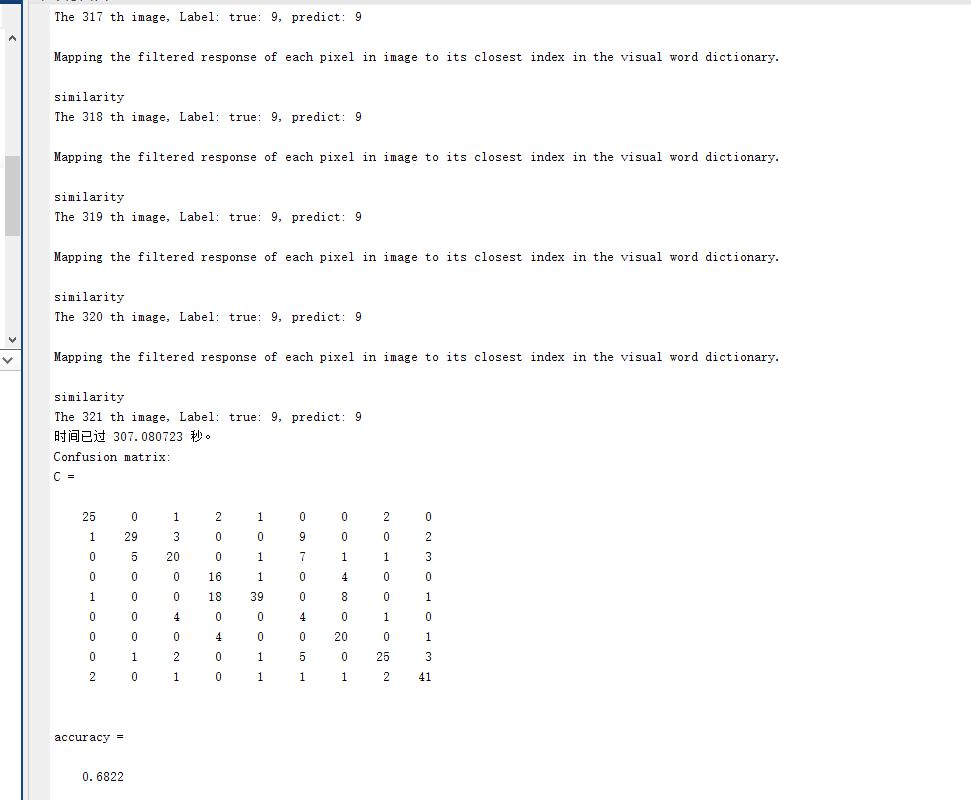
\includegraphics[width=0.9\linewidth]{./figures/k=25_sim.jpg} 
\end{figure}

\begin{table}[h!]
  \centering

  \begin{tabular}{|c|c|c|c|c|c|c|}
    \hline
    {\bf K} & {\bf 1} & {\bf 5} & {\bf 11} & {\bf 15} & {\bf 21} & {\bf 25} \\
    \hline
    {\bf Accuracy} & 0.5575 & 0.5888 & 0.6199 & 0.6262 & 0.6262 & {\bf 0.6822}\\
    \hline
  \end{tabular}
  \caption{{\bf Accuracy versus $k$ values.} Add some nice observations here!}
\end{table}

We found when $k$ increases, the accuracy also increases. But when $k$ gets large, the accuracy no longer changes.

A plot of $k$ \textit{v.s.} the classification accuracy (see Fig.~\ref{fig:q5_10_k}).

\begin{figure}[ht!]
	\caption{$k$ \textit{v.s.} the classification accuracy}
	\centering 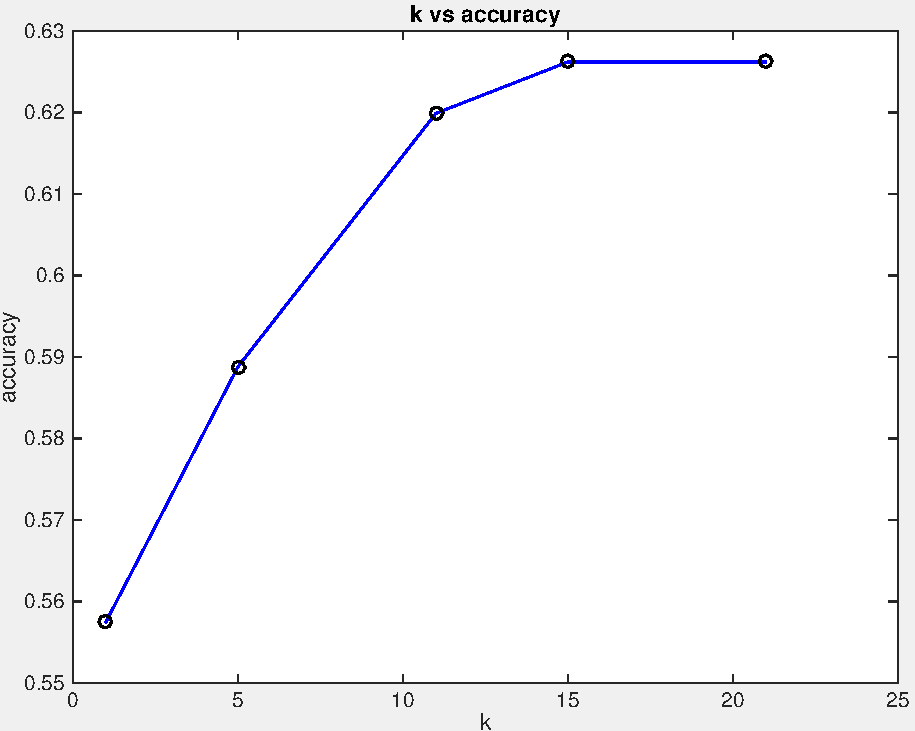
\includegraphics[width=0.9\linewidth]{./figures/k_vs_accuracy.pdf} 
	\label{fig:q5_10_k}
\end{figure}

Results of classification (see Fig.~\ref{fig:result_classification}).

\begin{figure}[htbp!]
\centering
	\begin{minipage}[t]{0.45 \textwidth}
		\centering 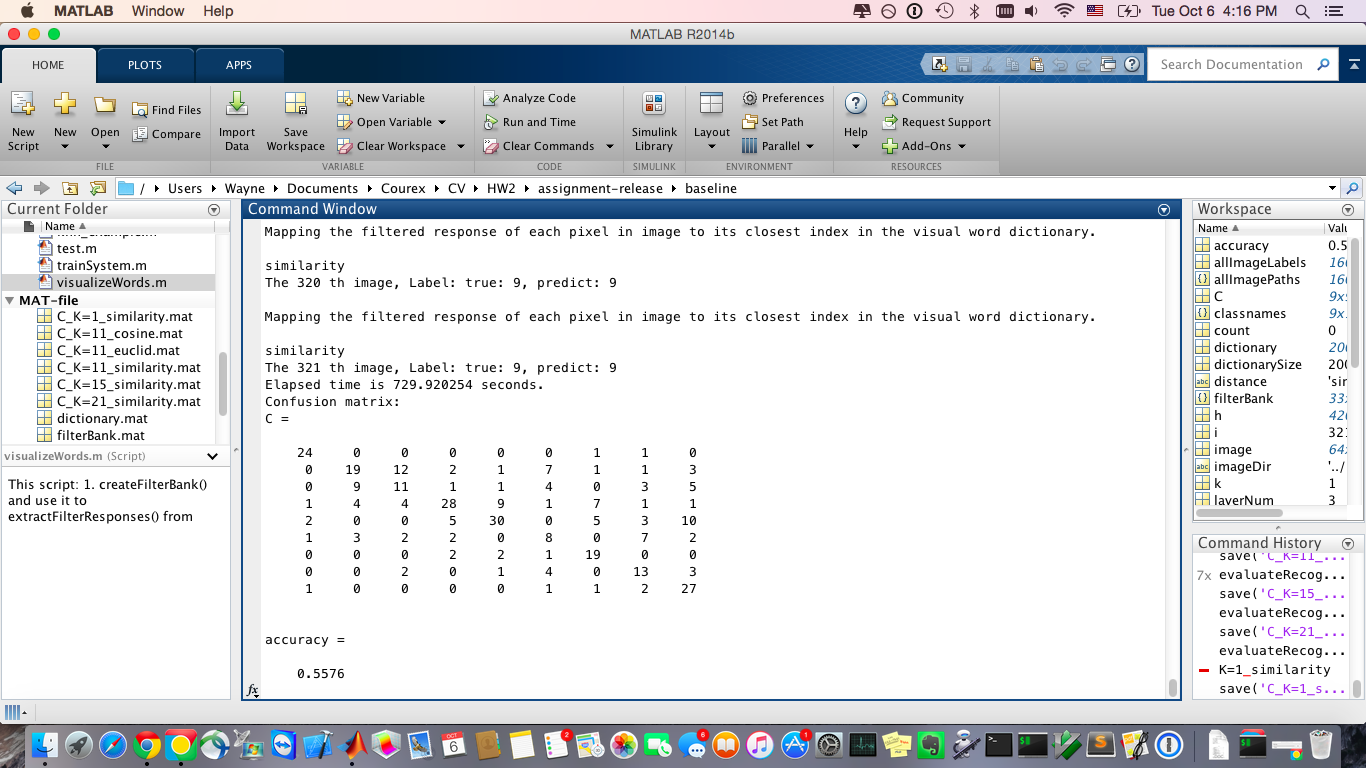
\includegraphics[width= \linewidth]{./figures/k=1_similarity} 
		\caption*{$k$=1}
	\end{minipage}
	\begin{minipage}[t]{0.45 \textwidth}
		\centering \includegraphics[width= \linewidth]{./figures/k=5_similarity} 
		\caption*{$k$=5}
	\end{minipage}
	\begin{minipage}[t]{0.45 \textwidth}
		\centering \includegraphics[width= \linewidth]{./figures/k=11_similarity} 
		\caption*{$k$=11}
	\end{minipage}
	\begin{minipage}[t]{0.45 \textwidth}
		\centering \includegraphics[width= \linewidth]{./figures/k=15_similarity} 
		\caption*{$k$=15}
	\end{minipage}
	\begin{minipage}[t]{0.45 \textwidth}
		\centering 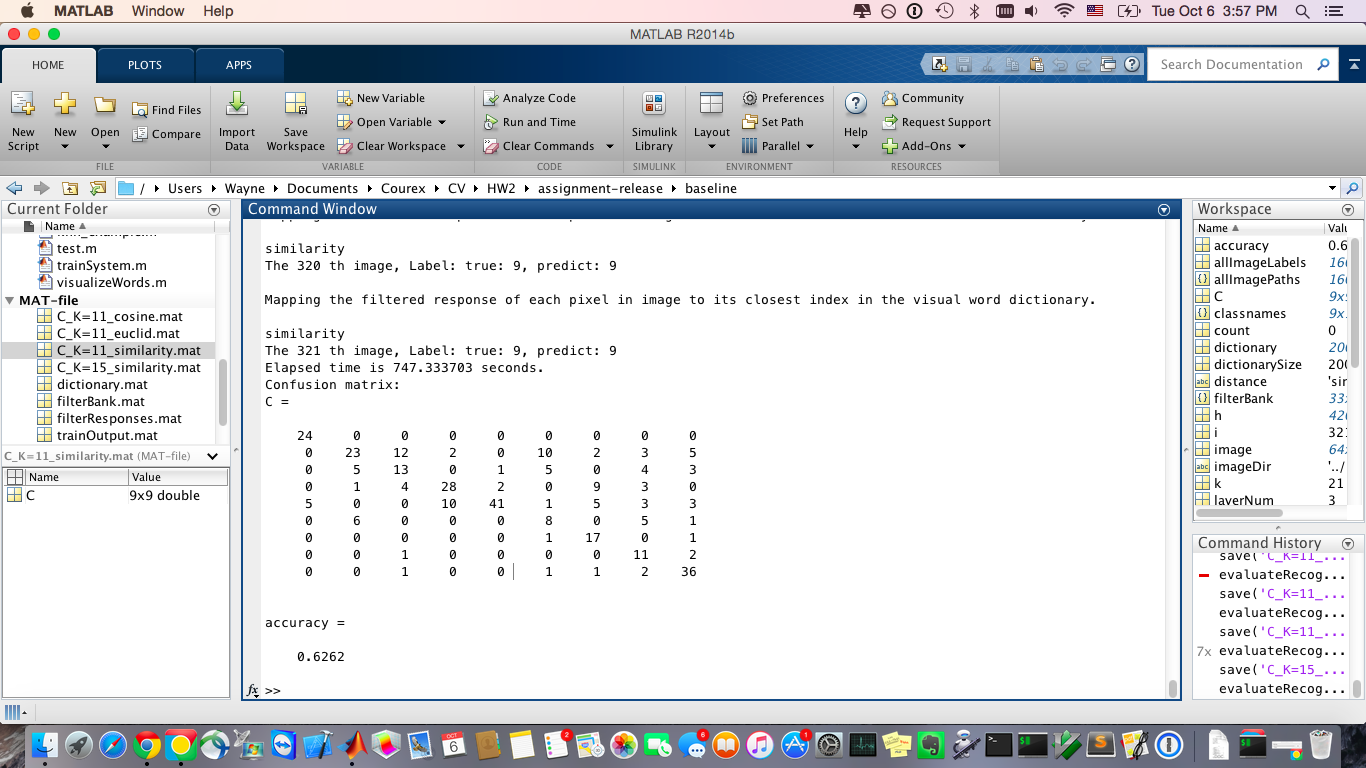
\includegraphics[width= \linewidth]{./figures/k=21_similarity} 
		\caption*{$k$=21}
	\end{minipage}
\caption{Results of classification.}
\label{fig:result_classification}
\end{figure}

\subsection{(5 pts, 2-3 lines): Theory}

Nearest neighbor method needs to compute the similarity of data vectors in the dataset. For a large dataset, we need to initialize many centers, and if the vector dimension is high, the computational cost increases. Besides, it does not uniquely weigh different distances.

\section{Final thoughts on visual words (40 pts)}

\subsection{(20 pts)}

Coding question, put your implementation in \verb+visualizeWords.m+


\lstinputlisting{./code/visualizeWords.m}

Add your figure here. See Fig.~\ref{fig:visual_words}.

\begin{figure}[ht!]
  \centering 
\includegraphics[width=0.8\linewidth]{./figures/visualwords}
  \caption{{\bf Visualization of words.} The visualization of one word is essentially searching all the images for pixel patches that have their center indexes mapped to this word. The basis idea is that for a pixel in the image that is categorized to a word in the dictionary, its surrounding pixels should at least close to this pixel. So summing up and average all the patches will give us a visual sense of what the word will look like.}
\label{fig:visual_words}
\end{figure}

\subsection{(10 pts)}

Add your explanation here with some nice pictures.

\noindent\textbf{Explanation:}
For the demonstration purpose, I choose three classes from the pool to visualize: bamboo, basilica and railroad. The classification accuracy (as shown in \ref{confusionMatrix}) for class \emph{bamboo} and \emph{basilica} is high, while for \emph{railroad} is low, and \emph{railroads} are much wrongly classified as \emph{basilica}. If we want high classification accuracy, we expect the words within class are similar while across classes are distinctive. We can see from Fig.~\ref{fig:top10}, that for \emph{bamboo}, its top 10 words looks similar. But for the latter two their top 10 words looks like they have somewhat unique patterns, especially for \emph{railroad}. Looking in the detail, we found for \emph{railroads} they have more word representations than others. This is due to the image set for \emph{railroad} has many distinctive changes (light, surroundings, etc). These words are of less representation to this class, but might more to classes that share similar words, say, \emph{basilica}. To overcome this problem, we can on the one hand enlarge the dataset or capture new features for this class to extract more generalized patterns, on the other hand reduce the cluster number of this class to avoid sensitiveness to noise.

\begin{figure}[!htbp]
\centering
  \begin{minipage}[t]{0.2 \textwidth}
    \centering 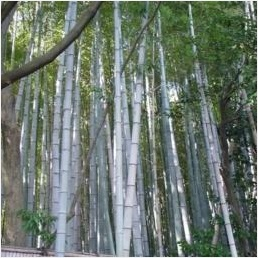
\includegraphics[width= \linewidth]{./figures/bamboo} 
    \centering 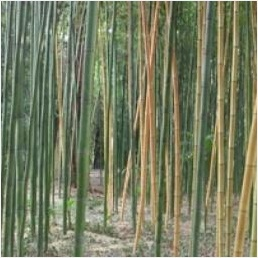
\includegraphics[width= \linewidth]{./figures/bamboo2} 
    \caption*{bamboo}
  \end{minipage}
  \begin{minipage}[t]{0.45 \textwidth}
    \centering 
\includegraphics[width= \linewidth]{./figures/bamboo_top10}
    \centering 
\includegraphics[width= \linewidth]{./figures/bamboo2_top10}  
    \caption*{top10}
  \end{minipage}

  \begin{minipage}[t]{0.2 \textwidth}
    \centering 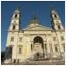
\includegraphics[width= \linewidth]{./figures/basilica} 
    \centering 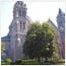
\includegraphics[width= \linewidth]{./figures/basilica2} 
    \caption*{basilica}
  \end{minipage}
  \begin{minipage}[t]{0.45 \textwidth}
    \centering 
\includegraphics[width= \linewidth]{./figures/basilica_top10} 
    \centering 
\includegraphics[width= \linewidth]{./figures/basilica2_top10} 
    \caption*{top10}
  \end{minipage}

  \begin{minipage}[t]{0.2 \textwidth}
    \centering 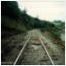
\includegraphics[width= \linewidth]{./figures/railroad}
    \centering 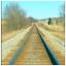
\includegraphics[width= \linewidth]{./figures/railroad2}  
    \caption*{railroad}
  \end{minipage}
  \begin{minipage}[t]{0.45 \textwidth}
    \centering 
\includegraphics[width= \linewidth]{./figures/railroad_top10}
    \centering 
\includegraphics[width= \linewidth]{./figures/railroad2_top10}  
    \caption*{top10}
  \end{minipage}
\caption{Top 10 words.}
\label{fig:top10}
\end{figure}

\begin{lstlisting}

\end{lstlisting}

\subsection{(10 pts, 4-5 lines): Dataset Expansion}
1. A way to expand the dataset without using external images is to extract new features from the same dataset. For instance, we can extract interest points features instead of filter-banked features.\\
2. Flipping will help in bag-of-words with spatial pyramid matching, but not in bag-of-words. Because the former respects spatial information of images, but the latter does not (see \ref{sub:bag-of-words}).

\section{Extra Credit: Boosting performance (45 pts)}

For the die-hards\ldots

\subsection{Better filter bank (10 pts)}
The first added is ``\emph{Gabor}'' filters, they pick up the local spatial and frequency information of images, and sensitive to the edges so that can captures edges of different directions and scales (textures). They are also adaptive to the change of light.

 The second added is ``\emph{Laplacian}'' filters, they pick up the second order derivative of an image isotropically. They are used to detect edges and sharpen the image, but sensitive to noise.

 (See Fig.~\ref{fig:filter_bank}.)

\begin{figure}
\centering
  \begin{minipage}[t]{0.8 \textwidth}
    \centering 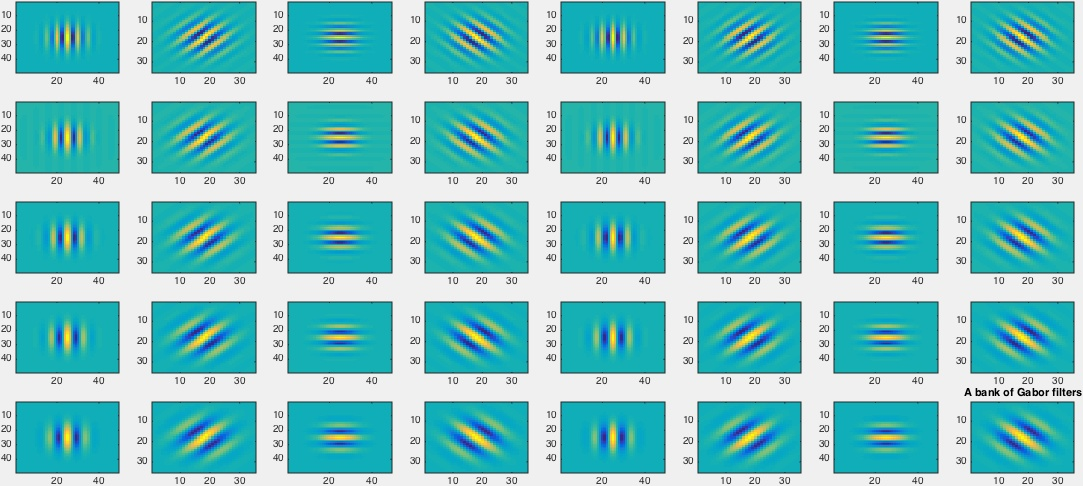
\includegraphics[width= \linewidth]{./figures/gaborBank} 
    \caption*{Gabor filter}
  \end{minipage}
  \begin{minipage}[t]{0.8 \textwidth}
    \centering 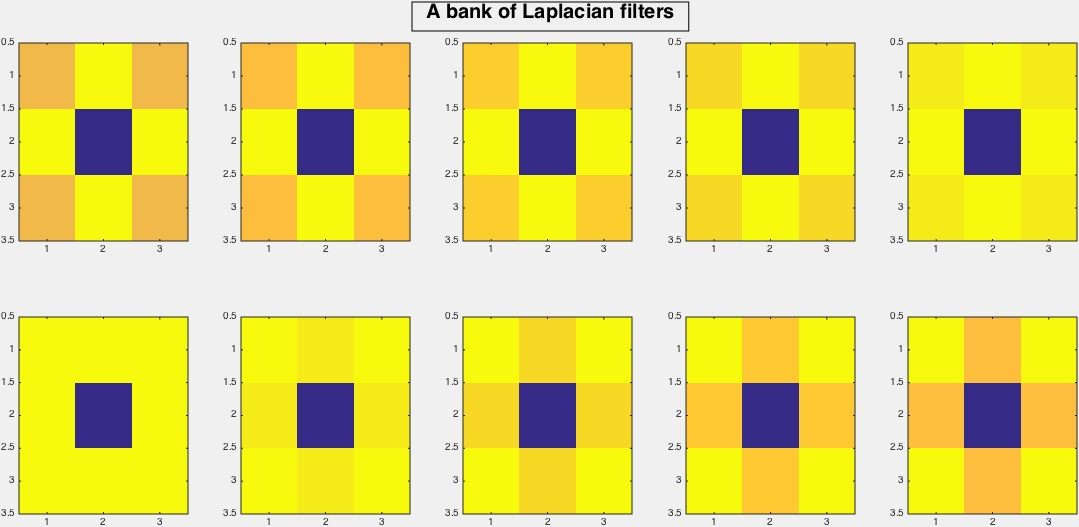
\includegraphics[width= \linewidth]{./figures/laplacianBank}
    \caption*{Laplacian filter}
  \end{minipage}
\caption{Additional filter banks.}
\label{fig:filter_bank}
\end{figure}

\subsection{Better image similarity function (5 pts)}
I tried \emph{Euclidean} distance and \emph{Cosine} distance for \emph{KNN} classification. 

The distance \emph{v.s} accuracy table is shown below in Tab.~\ref{tab:acc_vs_diff_dis}.

\begin{table}[h!]
  \centering

  \begin{tabular}{|c|c|c|c|}
    \hline
    {\bf Distance} & {\bf Similarity} & {\bf Euclidean} & {\bf Cosine}  \\
    \hline
    {\bf Accuracy} & 0.6199 & 0.4112 & 0.3988 \\
    \hline
  \end{tabular}
  \caption{{\bf Accuracy versus different distances.} ($k=11$)}
\label{tab:acc_vs_diff_dis}
\end{table}

Code for switching from different choice of distances:

\begin{lstlisting}
switch lower(choiceDistance)
    case 'similarity'
        % - similarity
        dist = distanceToSet(testSet, trainSet); % similarity in this case
        [dist_sort, pos]= sort(dist, 'descend'); % sort the distance in descending order and mark the position
        distance = dist_sort(1:K); % find the top K distances...
        neighbor = trainLabel(pos(1:K)); % and their corresponding labels in trainSet
    case 'euclid'
        % - Euclid distance
        dist = pdist2(testSet.', trainSet.', 'euclid');
        [dist_sort, pos]= sort(dist, 'ascend');
        distance = dist_sort(1:K);
        neighbor = trainLabel(pos(1:K));
    case 'cosine'
        % - Cosine distance
        dist = pdist2(testSet.', trainSet.', 'cosine');
        [dist_sort, pos]= sort(dist, 'ascend');
        distance = dist_sort(1:K);
        neighbor = trainLabel(pos(1:K));
    case 'kldivergence'
        % - K-L divergence
        KL = @(X, Y)(sum(bsxfun(@times, X, bsxfun(@minus, log2(X),log2(Y)))));
        dist = pdist2(testSet,trainSet, @(testSet,trainSet) KL(testSet,trainSet));
        [dist_sort, pos]= sort(dist, 'ascend');
        distance = dist_sort(1:K);
        neighbor = trainLabel(pos(1:K));
    case 'builtinknn'
        [idx, dist] = knnsearch(trainSet.',testSet.', 'dist','euclid','k',K);
        distance = dist;
        neighbor = trainLabel(idx);
    otherwise
        disp('Undefined distance!\n');
end
\end{lstlisting}

\subsection{Different Features (15 pts)}
I tried using SURF descriptors to get the visual word dictionary and mapping images to word maps. The dictionary size is set to 500.

Then the histograms were got as features for classification \emph{WITHOUT} using SPM.

The accuracy is: \emph{0.3396} (see Fig.~\ref{fig:knn_surf}).

\begin{figure}[ht!]
  \centering 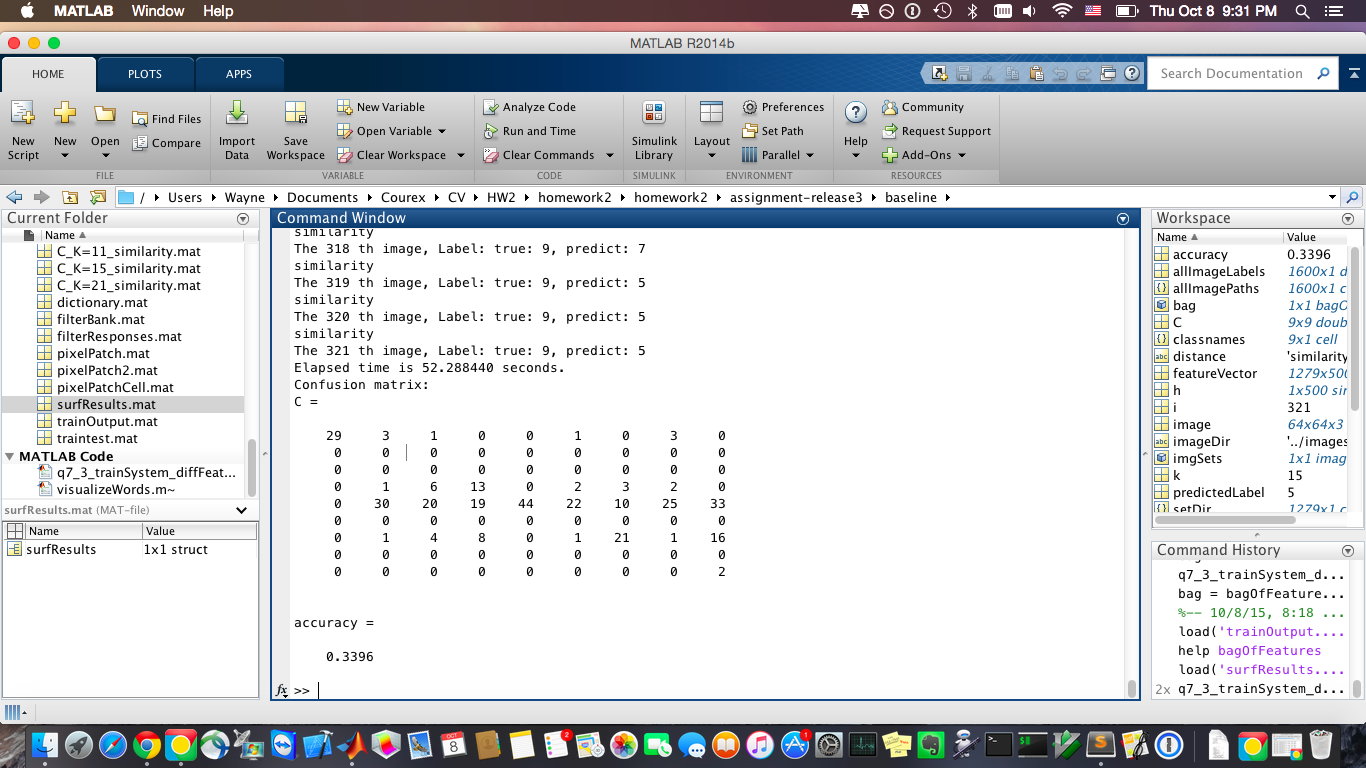
\includegraphics[width=0.8\linewidth]{./figures/K=15_surf}
  \caption{{\bf KNN result using SURF-bag-of-words.} (K=15)}
  \label{fig:knn_surf}
\end{figure}  

The code is shown below:
\lstinputlisting{./code/q7_3_trainSystem_diffFeatures.m}

\subsection{Encoding (15 pts)}
A \emph{`soft-histogram'} is used to encode the features to visual word dictionary\cite{ahonen2007soft}, in which:

Instead of assigning one feature to a hard one visual word, a membership between (0,1) is used to measure the belongingness to a certain dictionary. 

The membership is computed as:
\[ U_k = (1/\|X-d_k\|^2_2)/\sum(1/\|X-d_k\|^2_2) \]

code:
\lstinputlisting{./code/softHist.m}

\subsection{Getting Fancy! (0 pts)}
\emph{I can use SVMs to do classification, but since there is 0 pts...}

\bibliographystyle{ieeetr} 
\bibliography{bib1}

\end{document}
